\documentclass[
	parskip=half,
	a4paper,
]{scrarticle}

\usepackage{xcolor}
\definecolor{seeblau}{HTML}{00A9E0}
\definecolor{seegrau}{HTML}{9AA0A7}

\definecolor{seeblau1}{HTML}{CCEEF9}
\definecolor{seeblau2}{HTML}{A6E1F4}
\definecolor{seeblau3}{HTML}{59C7EB}
\definecolor{seeblau4}{HTML}{00A9E0}
\definecolor{seeblau5}{HTML}{008ECE}


\usepackage{graphicx}
\usepackage{amsmath}
\usepackage{subcaption}
\usepackage{wrapfig}
\usepackage[english]{babel}
\usepackage{blindtext}
\usepackage{microtype}
\usepackage{siunitx}
\usepackage[utf8]{inputenc}
\usepackage{csquotes}
\usepackage{nicefrac}
\usepackage[T1]{fontenc}
\usepackage{amsfonts}
\usepackage{amssymb}
\usepackage{tikz}
\usepackage{parskip}

\usepackage{libertinus, libertinust1math}
\usepackage[sfdefault]{biolinum}
\usepackage{roboto}

\setkomafont{disposition}{\normalfont\sffamily}

% set margins
\usepackage{geometry}
\geometry{
	a4paper,
	left=2.5cm,
	right=2.5cm,
	top=2.5cm,
	bottom=2.5cm
}

% caption
\usepackage{caption}
\captionsetup{
	% font={sf},
	labelfont={sf, bf, color=seeblau},
	labelsep=quad,
	labelformat=simple,
}

% links
\usepackage{hyperref}
\hypersetup{
	colorlinks=true,
	linkcolor=seeblau,
	citecolor=seeblau,
	urlcolor=seeblau,
	% hidelinks=true
}

% bibliography
\usepackage[
	style=numeric-comp, % comp = compressed 4,5,6,7 -> 4-7
	sorting=none,		% Sort by appearance
	% autocite = superscript,
	% backref=true,
	hyperref=true,
	url=true,
	maxbibnames=100
]{biblatex}

\usepackage{float}
% \floatplacement{figure}{h}
% \floatplacement{table}{H}

% loosen float placement rules
\renewcommand{\topfraction}{0.8}
\renewcommand{\bottomfraction}{.8}
\renewcommand{\textfraction}{0.1}
\renewcommand{\floatpagefraction}{.9}
% make floats less likely to be placed on a separate page
\setcounter{totalnumber}{9}
\setcounter{topnumber}{9}
\setcounter{bottomnumber}{9}

% decrease space between floats and text
\setlength{\textfloatsep}{0.25cm}
\setlength{\floatsep}{0.25cm}

% decrease space after disposition
\RedeclareSectionCommands[
	afterskip=1px
]{section, subsection, subsubsection}

\usepackage{adjustbox}

\usepackage{datetime}
\newdateformat{dotdate}{
	\twodigit{\THEDAY}.\twodigit{\THEMONTH}.\THEYEAR
}
\newdateformat{monthyeardate}{%
  \monthname[\THEMONTH] \THEYEAR}


% header and footer
\usepackage[
  markcase=noupper
]{scrlayer-scrpage}% activates pagestyle scrheadings automatically
\clearpairofpagestyles
\setkomafont{pageheadfoot}{\normalfont\sffamily}
\setkomafont{pagenumber}{\normalfont\sffamily}
% \chead*{\color{seegrau} Draft \dotdate\today}
\ofoot*{\pagemark}
\ohead*{\rightmark}


\usepackage{ifthen}
\newcommand{\markieren}[4]{
	\ifthenelse{\equal{#1}{}}{}{\adjustbox{padding=3pt, bgcolor=seeblau1, margin=-1pt}{\strut{\sffamily\robotoMedium{#1}}}\\}
  \ifthenelse{\equal{#2}{}}{}{\adjustbox{padding=3pt, bgcolor=seeblau2, margin=-1pt}{\strut{\sffamily\robotoMedium{#2}}}\\}
	\ifthenelse{\equal{#3}{}}{}{\adjustbox{padding=3pt, bgcolor=seeblau3, margin=-1pt}{\strut{\sffamily\robotoMedium{#3}}}\\}
	\ifthenelse{\equal{#4}{}}{}{\adjustbox{padding=3pt, bgcolor=seeblau4, margin=-1pt}{\strut{\sffamily\robotoMedium{#4}}}}
}

\addbibresource{../literature.bib}
\begin{document}

\title{Procedures for Hot Electron Measurements}
\author{Leon Oleschko}
\date{\dotdate\today}

\begin{titlepage}
    \sffamily
    \vspace*{3cm}
    {
        \fontsize{32}{32}
        \markieren{}{Hot Electron}{Thermal Emission}{Spectroscopy}
    }
    \vspace{.25cm}\\
    {
        \Large
        Leon Oleschko\\
        Supervised by Peter Baum
        \vspace{.05cm}\\
        \dotdate\today\\
        % \vspace{.25cm}\\
        % \normalsize
        Universität Konstanz
    }
    \vfill
    {
        \normalfont\normalsize

    }
    \vfill
    \begin{flushright}
        Available at \url{www.github.com/leoole100/projekt-praktikum}.
    \end{flushright}
\end{titlepage}

% {
% 	\sffamily
% 	\hypersetup{hidelinks}
% 	\tableofcontents
% }

\clearpage


\addcontentsline{toc}{section}{Introduction}
\section*{Introduction}

\section{Experimental Setup}
The experimental setup, originally designed by Leon Roob \autocite{roob_thermal_2025}, enables measurement of thermal radiation from ultrafast hot electrons. It follows the principles of typical ultrafast photoemission spectroscopy \autocite{lui_ultrafast_2010}, combining femtosecond laser excitation with precise collection optics and spectral detection. Thermal emission from the sample is collected by parabolic mirrors and analysed using a monochromator equipped with a blazed diffraction grating, with detection performed by an EMCCD camera. The following sections describe the collection optics, the monochromator, and the detector in more detail.


\subsection{Collection}
Thermal radiation emitted by the excited hot electrons is collected using two off-axis parabolic aluminium mirrors. The first parabolic mirror (PM1), with a diameter of \SI{50.8}{\milli\meter} and a focal length of \SI{50.8}{\milli\meter}, collimates the emitted light from the sample. A second parabolic mirror (PM2), structurally identical but with a focal length of \SI{101.6}{\milli\meter}, focuses the collimated radiation into an optical fibre leading to the monochromator. This geometry ensures efficient light collection over a broad solid angle, which is critical given the low photon flux characteristic of ultrafast thermal emission measurements.

To suppress residual laser fundamental radiation, two Schott KG3 infrared filters are placed between PM2 and the fibre input. These filters exhibit high transmittance between \SI{360}{\nano\meter} and \SI{590}{\nano\meter} but attenuate light outside this range to less than \SI{0.1}{\percent}. Both filters are tilted to prevent back reflections into the optical path, though this tilt reduces their maximum transmission to around \SI{20}{\percent} per filter for visible wavelengths. Transmission losses from filters and mirror coatings must be accounted for during system calibration to accurately reconstruct the emission spectrum.

\subsection{Monochromator}
The spectrally resolved analysis of the collected thermal radiation is performed using an Acton SpectraPro 300i monochromator. This instrument employs a ruled diffraction grating with 150 grooves per millimetre and a blaze wavelength of 500 nm. The blazing optimises the grating's diffraction efficiency for visible wavelengths near the blaze wavelength, while efficiency drops off at shorter or longer wavelengths. This wavelength-dependent efficiency curve is a critical factor influencing the measured spectra and must be corrected during calibration procedures to achieve accurate spectral intensity measurements.

The monochromator allows tuning of the central wavelength and control of the spectral bandwidth through adjustable entrance and exit slits. The selection of slit widths is a trade-off between spectral resolution and photon throughput, which is particularly important for weak signals from ultrafast thermal emission.

\subsection{Detector}
Spectrally dispersed thermal radiation is detected using an Andor iXonEM+ CCD camera. Although this camera features an electron multiplication (EM) register capable of amplifying low-light signals, in this setup the EM feature is disabled. Initial tests showed that electron multiplication introduced excess noise, ultimately reducing the signal-to-noise ratio (SNR). Instead, measurements are performed in conventional CCD mode, which provides better overall sensitivity for the photon flux levels encountered in thermal emission experiments.

The detector's quantum efficiency peaks in the visible spectral range but drops significantly below approximately 480 nm, as specified in the manufacturer's datasheet \autocite{andor_ixonem_nodate}. This wavelength-dependent response must be considered when analysing measured spectra, and corrections may be required to reconstruct the true emission profile. In addition, variations in quantum efficiency between individual cameras can introduce systematic errors, highlighting the need for in-situ calibration to ensure quantitative accuracy.


\section{Noise Sources and SNR Optimisation}

The detector response is fundamentally linear, meaning the measured signal is directly proportional to the incoming photon flux and exposure time. However, the signal is offset by an electronic bias level, which is added to avoid negative values during digitisation. This offset can be easily removed by subtracting a bias frame acquired with the same settings but without illumination.\\
Beyond this deterministic offset, there are statistical fluctuations in the pixel signal, collectively referred to as noise. These noise contributions are not constant but depend on several parameters of the measurement, such as readout settings, exposure time, sensor temperature, and gain. For a measured signal the total noise can be estimated as

\begin{equation}
    \sigma_{\text{total}} = \sqrt{\sigma_{\text{read}}^2 + \sigma_{\text{dark}}^2 + \sigma_{\text{shot}}^2 + \sigma_{\text{CIC}}^2}.
\end{equation}

\paragraph{Readout Noise}

Readout noise arises during charge-to-voltage conversion and digitisation in the detector electronics. It is essentially constant for a given readout mode and independent of the exposure time or photon flux. Without electron multiplication (EM) gain, this noise typically amounts to $2$--$5~e^{-}$~RMS. An important consideration is that readout noise scales \emph{per readout bin}. Summing multiple pixels via hardware binning before digitisation can significantly reduce the overall noise, as only a single readout noise contribution is added for the binned superpixel rather than for each individual pixel. Hardware binning is therefore advisable wherever spatial or spectral resolution permits.

In EM mode, the effective readout noise is reduced because the signal is amplified before readout. However, this benefit comes at the cost of introducing other noise contributions, such as clock-induced charge.

\paragraph{Thermal Noise (Dark Current Noise)}

Thermal noise, or dark current noise, originates from thermally generated electrons accumulating in each pixel during the exposure time. It scales with both temperature and exposure time, following Poisson statistics:

\begin{equation}
    \sigma_{\text{dark}} = \sqrt{I_{\text{dark}} \cdot t_{\text{exp}}},
\end{equation}

where $I_{\text{dark}}$ is the dark current in electrons per second per pixel, and $t_{\text{exp}}$ is the exposure time. The dark current itself depends exponentially on the sensor temperature:

\begin{equation}
    I_{\text{dark}}(T) = I_0 \cdot \exp\left(-\frac{E_{\text{gap}}}{k T}\right),
\end{equation}

where $I_0$ is a device-specific pre-exponential factor, $E_{\text{gap}}$ is the effective activation energy (typically around $0.6$--$0.7$~eV for silicon), $k$ is the Boltzmann constant, and $T$ is the absolute temperature in Kelvin. This exponential relationship underscores the importance of sensor cooling to minimise dark noise in low-light measurements.

Figure~\ref{fig:dark_noise} shows the measured dark noise as a function of sensor temperature and exposure time, along with a fit using the exponential model for $I_{\text{dark}}$.

\begin{figure}
    \centering
    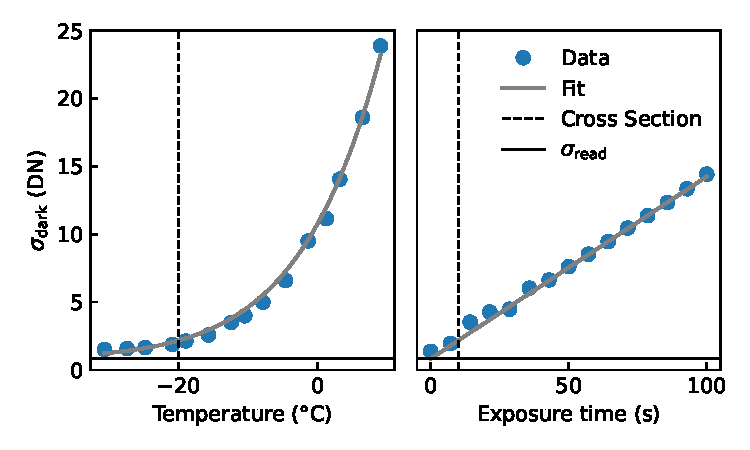
\includegraphics{../analysis/figures/dark_noise.pdf}
    \caption{Dark noise as a function of sensor temperature and exposure time. The curve is fitted with an effective activation energy of $E_\text{gap} = \SI{0.597(4)}{eV}$ and a constant readout noise of $\sigma_{\text{read}} = \SI{0.81(12)}{e^-}$.}
    \label{fig:dark_noise}
\end{figure}

\paragraph{Shot Noise}

Shot noise arises from the discrete nature of photon arrival and follows Poisson statistics. It scales with the square root of the signal:

\begin{equation}
    \sigma_{\text{shot}} = \sqrt{S}.
\end{equation}

Although shot noise cannot be eliminated, its relative impact decreases as the total signal increases, since the signal-to-shot-noise ratio improves proportionally to $\sqrt{S}$.

\paragraph{Clock-Induced Charge (CIC)}

Clock-induced charge (CIC) is a noise source unique to EM gain mode. It originates from spurious electrons generated during rapid voltage transitions as charges are shifted through the EM register. CIC is essentially independent of exposure time and becomes significant for short exposures and low-light conditions when using high EM gain. The noise contribution from CIC can be approximated as

\begin{equation}
    \sigma_{\text{CIC}} = \sqrt{N_{\text{CIC}} \times \text{EM}_{\text{gain}}^2},
\end{equation}

where $N_{\text{CIC}}$ is the average number of CIC electrons per pixel per frame, and $\text{EM}_{\text{gain}}$ is the electron multiplication gain factor. While EM gain reduces readout noise, it also amplifies CIC and introduces multiplicative noise (with an excess noise factor around $\sqrt{2}$), which can degrade the overall signal-to-noise ratio (SNR) in low-light measurements.

\paragraph{Implications for SNR Optimisation}

These different noise sources scale differently with experimental parameters. While readout noise is essentially constant, dark noise increases with exposure time and temperature. Shot noise increases with the square root of the signal, whereas CIC becomes significant primarily in EM gain mode and short exposures.

In practice, lower EM gain and longer exposure times are generally beneficial for achieving higher SNR because they increase the collected signal and reduce the relative impact of frame-based noise contributions like CIC. However, longer exposures also increase dark noise, which necessitates effective cooling. In the measurements performed for this work, the electron multiplication feature of the Andor iXonEM+ camera was disabled. Tests showed that EM gain introduced significant additional noise, including CIC, which degraded the overall SNR. Therefore, data acquisition was carried out in conventional CCD mode, using longer exposure times, sensor cooling, and hardware binning where possible to optimise sensitivity while maintaining acceptable noise levels.

\subsection{Calculating the expected SNR}
To demonstrate how the understanding of the System Noise can be used the SNR of the Hot Electron Experiment is being calculated.
The signal strength should be in the order of $10^{-9}\;\si{W/nm}$ and centered around $\lambda = \SI{600}{nm}$. Let's say we want to have a spectral resolution of \SI{1}{nm}. This means that we need to detect a signal of $P=10^{-9}\;\si{W}$. This means $P \lambda / hc = \SI{2.5e-9}{Hz}$ Photons per second.


\section{Efficiency and Flatness}
After light is generated as thermal radiation with a spectral power distribution $B(\lambda)\, d\lambda$ on a piece of the surface of the sample with radius $r_0$, it is emitted with a radial distribution. For simplicity, it is assumed to be omnidirectional.

The collection mirror (PM1) captures a fraction of this radiation determined by its solid angle $\Omega$ as seen from the emission point. For a circular mirror of radius $r_\text{PM}$ positioned at a distance $f_\text{PM}$ (the focal length), the collection half-angle $\theta$ is given by

\begin{equation}
    \theta = \arctan\left( \frac{r_\text{PM}}{f_\text{PM}} \right).
\end{equation}

The solid angle subtended by the mirror is then

\begin{equation}
    \Omega = 2\pi \left( 1 - \cos \theta \right).
\end{equation}

Relative to the total spherical emission of $4\pi$ steradians, the fraction of thermal radiation collected is

\begin{equation}
    f_\Omega = \frac{\Omega}{4\pi}.
\end{equation}

Hence, the spectral power captured by PM1 is

\begin{equation}
    P_\text{PM1}(\lambda) 
    = B(\lambda) \cdot A_\text{emit} \cdot f_\Omega,
\end{equation}

where $A_\text{emit} = \pi r_0^2$ is the area of the emitting region on the sample.

The collimated light is subsequently directed toward the second parabolic mirror (PM2), which focuses it into a spot of diameter $d_\text{focus}$ determined by the system magnification $M$:

\begin{equation}
    M = \frac{f_\text{PM2}}{f_\text{PM1}},
\end{equation}

yielding

\begin{equation}
    d_\text{focus} = M \cdot 2 r_0.
\end{equation}

However, the optical fibre used as the spectrometer entrance has a core diameter $d_\text{fibre} = \SI{200}{\micro\meter}$. Therefore, only a fraction of the focused light is coupled into the fibre, given by the ratio of their areas:

\begin{equation}
    f_\text{fibre, area}
    =
    \left( \frac{d_\text{fibre}}{d_\text{focus}} \right)^2.
\end{equation}

Furthermore, the fibre's numerical aperture (NA) limits the acceptance angle of incoming rays. Assuming the focused beam has a divergence $\theta_\text{beam}$ smaller than the fibre's acceptance angle, the angular coupling efficiency $f_\text{NA}$ can be approximated as unity. If not, an additional loss factor must be included. The fibre's acceptance angle can be improved by using a cosine corrector, but this introduces additional losses.

Losses within the fibre itself are considered negligible.

The light then reaches the monochromator, where again there may be a mismatch between the NA of the first monochromator mirror and the fibre, resulting in further losses.

The losses in the mirrors are small and can be neglected in this analysis.

The main contributions to the wavelength-dependent transmission curve through the spectrometer and the entire setup are:

\begin{equation}
    T_\text{optics}(\lambda) 
    \propto T_\text{filters}(\lambda)
    \times T_\text{grating}(\lambda)
    \times \text{QE}(\lambda),
\end{equation}

where:

\begin{itemize}
    \item $T_\text{filters}(\lambda)$ represents the transmission of short-pass or band-pass filters,
    \item $T_\text{grating}(\lambda)$ is the blazing efficiency of the monochromator grating,
    \item $\text{QE}(\lambda)$ is the quantum efficiency of the detector.
\end{itemize}

Hence, the spectral power density finally detected by the EMCCD is

\begin{equation}
    P_\text{detected}(\lambda)\, d\lambda
    = B(\lambda)\, d\lambda \cdot A_\text{emit} \cdot f_\Omega 
      \cdot f_\text{fibre, area} 
      \cdot f_\text{NA}
      \cdot T_\text{optics}(\lambda).
\end{equation}

Expressing this as a detected photon rate for a wavelength interval $[\lambda, \lambda + d\lambda]$ requires dividing by the photon energy $E_\text{photon}(\lambda)$:

\begin{equation}
    N_\text{photons}(\lambda, d\lambda)
    = \frac{P_\text{detected}(\lambda)\, d\lambda}{E_\text{photon}(\lambda)},
\end{equation}

where

\begin{equation}
    E_\text{photon}(\lambda)
    = \frac{h c}{\lambda}.
\end{equation}

\subsection{Measurement of the Sensitivity Curve}

The wavelength-dependent sensitivity of the entire optical system is described by the \emph{sensitivity curve}, also referred to in the literature as the \emph{throughput curve}, \emph{efficiency curve}, or \emph{instrument response curve}. This curve represents the combined wavelength-dependent transmission and detection efficiency of all optical components in the setup, including filters, the diffraction grating, fibre coupling, and the detector's quantum efficiency. Accurate determination of the sensitivity curve is essential for converting measured spectra into absolute spectral power distributions emitted by the sample.

One common approach for determining the sensitivity curve is a direct measurement using a calibrated broadband light source. A lamp with a well-characterized spectral emission is coupled directly into the entrance fibre of the spectrometer. The spectrum recorded by the spectrometer is then compared to the lamp's certified spectral output. The sensitivity curve is obtained as the ratio of the measured signal to the known lamp spectrum, corrected for any geometrical factors such as fibre coupling efficiency or beam divergence. This method provides an absolute calibration, but it requires a lamp with stable and precisely known spectral characteristics, as well as careful alignment to avoid additional systematic errors.

Another practical method is transfer calibration using a reference spectrometer. In this approach, the same calibrated lamp is first measured with a well-characterized reference spectrometer whose response is already known. The lamp spectrum is then measured with the experimental spectrometer under identical conditions. Dividing the spectrum obtained from the experimental spectrometer by that from the reference spectrometer yields the relative sensitivity curve. Although this method typically does not yield an absolute calibration without additional scaling, it is particularly useful when an absolute-calibrated lamp is unavailable but a reliable reference spectrometer is accessible.

A more sophisticated technique involves the use of a bolometer and a reference spectrometer, typically employed in calibration laboratories. A bolometer can measure the absolute radiant power across a broad spectral range with high accuracy, particularly when used in conjunction with a monochromator to isolate narrow wavelength intervals. Comparing the spectrometer's measured signal to the bolometric measurement allows for the derivation of an extremely accurate sensitivity curve, accounting for slit widths, spectral responsivity, and absolute radiometric units. However, this method is complex and requires access to specialized equipment, including a second monochromator and a precisely calibrated flat-response bolometer, making it impractical for routine laboratory calibrations.

In this work, the sensitivity curve was estimated based on the individual transmission and efficiency curves of the components used in the optical path. The quantum efficiency of the detector was obtained from manufacturer data \cite{andor_ixonem_nodate}, while the blazing efficiency of the monochromator grating was estimated using models available in the literature \cite{barker_ripple_1984}. The transmission curve of the optical filters was measured directly using a broadband white light source. These combined curves, shown in Figure~\ref{fig:transmission}, provide an estimated sensitivity curve that serves as the basis for correcting measured spectra and reconstructing the absolute spectral power distribution emitted by the sample.

\begin{figure}
    \centering
    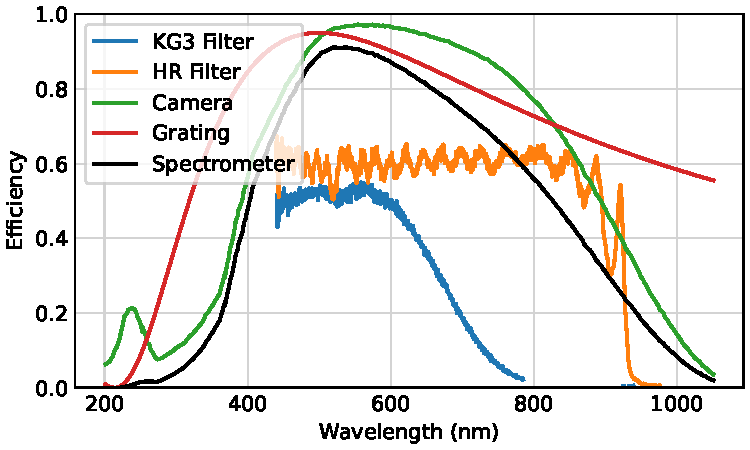
\includegraphics{../analysis/figures/filter.pdf}
    \caption{Transmission curves of various components and filters used in the setup.}
    \label{fig:transmission}
\end{figure}

 


\addcontentsline{toc}{section}{Concolusion}
\section*{Conclusion}

\clearpage
\printbibliography

\end{document}